\documentclass[a4paper]{article}
\usepackage{graphicx}
\usepackage[utf8]{inputenc}
\usepackage[english, serbian]{babel}

\title{UseCase dijagram: Podešavanja časopisa}
\date{09.11.2018.}
\author{Nadežda}

\begin{document}

\maketitle
\newpage

\begin{itemize}
    \item Naziv: Promena podešavanja časopisa
    \item Akter: Administrator sistema
    \item Kratak opis: Administrator menja podešavanja časopisa
    \item Osnovni tok događaja:(ponavljati korak 2 željeni broj puta)
        \begin{enumerate}
            \item Administrator pristupa obrascu za menjanje podataka
            \item Administrator unosi podatke u formu
            \item Adminstrator pokušava da sačuva nove podatke
            \item Novi podaci su sačuvani na sistemu
        \end{enumerate}
    \item Alternativni tok događaja:
        \begin{enumerate}
            \item Sistem ne može da sačuva nove podatke
                \begin{enumerate}
                    \item Administrator proverava da li su podaci validni u odnosu na već definisanu bazu podataka. Ponovo pokušava da sačuva podatke, ako ne uspe, prelazi na korak 1.b. alternativnog toka 
                    \item Administrator proverava internet konekciju i uspešno je podešava. Ponovo pokušava da sačuva podatke, ako ne uspe, prelazi na korak 1.c alternativnog toka
                    \item Administrator proverava da li je funkcionalnost slanja podataka preko forme dobro implementirana. Ako nije, popravlja to i pokušava ponovo da sačuva podatke. Ako ne uspe, prelazi na korak 1.d alternativnog toka
                    \item Ozbiljna greška sistema. Administrator traži grešku i pokušava da je otkloni.
                \end{enumerate}
        \end{enumerate}
\end{itemize}

\begin{figure}
    \centering
    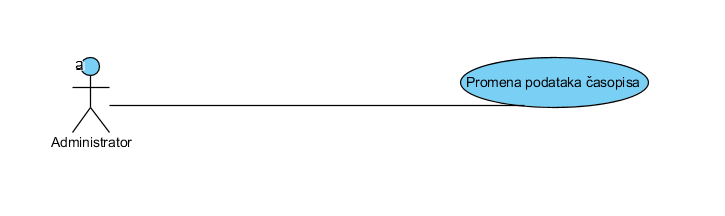
\includegraphics[width=\linewidth]{USeCasePromenaPodatakaCasopisa.png}
    \caption{UseCase screenshot}
    \label{fig:my_label}
\end{figure}


\end{document}